

%%%%%%%%%%%%%%%%%%%% book.tex %%%%%%%%%%%%%%%%%%%%%%%%%%%%%
%
% sample root file for the chapters of your "monograph"
%
% Use this file as a template for your own input.
%
%%%%%%%%%%%%%%%% Springer-Verlag %%%%%%%%%%%%%%%%%%%%%%%%%%


% RECOMMENDED %%%%%%%%%%%%%%%%%%%%%%%%%%%%%%%%%%%%%%%%%%%%%%%%%%%
\documentclass[graybox,envcountchap,sectrefs]{SpringerStyleFiles/styles/svmono}\usepackage[]{graphicx}\usepackage[]{color}
%% maxwidth is the original width if it is less than linewidth
%% otherwise use linewidth (to make sure the graphics do not exceed the margin)
\makeatletter
\def\maxwidth{ %
  \ifdim\Gin@nat@width>\linewidth
    \linewidth
  \else
    \Gin@nat@width
  \fi
}
\makeatother

\definecolor{fgcolor}{rgb}{0.345, 0.345, 0.345}
\newcommand{\hlnum}[1]{\textcolor[rgb]{0.686,0.059,0.569}{#1}}%
\newcommand{\hlstr}[1]{\textcolor[rgb]{0.192,0.494,0.8}{#1}}%
\newcommand{\hlcom}[1]{\textcolor[rgb]{0.678,0.584,0.686}{\textit{#1}}}%
\newcommand{\hlopt}[1]{\textcolor[rgb]{0,0,0}{#1}}%
\newcommand{\hlstd}[1]{\textcolor[rgb]{0.345,0.345,0.345}{#1}}%
\newcommand{\hlkwa}[1]{\textcolor[rgb]{0.161,0.373,0.58}{\textbf{#1}}}%
\newcommand{\hlkwb}[1]{\textcolor[rgb]{0.69,0.353,0.396}{#1}}%
\newcommand{\hlkwc}[1]{\textcolor[rgb]{0.333,0.667,0.333}{#1}}%
\newcommand{\hlkwd}[1]{\textcolor[rgb]{0.737,0.353,0.396}{\textbf{#1}}}%
\let\hlipl\hlkwb

\usepackage{framed}
\makeatletter
\newenvironment{kframe}{%
 \def\at@end@of@kframe{}%
 \ifinner\ifhmode%
  \def\at@end@of@kframe{\end{minipage}}%
  \begin{minipage}{\columnwidth}%
 \fi\fi%
 \def\FrameCommand##1{\hskip\@totalleftmargin \hskip-\fboxsep
 \colorbox{shadecolor}{##1}\hskip-\fboxsep
     % There is no \\@totalrightmargin, so:
     \hskip-\linewidth \hskip-\@totalleftmargin \hskip\columnwidth}%
 \MakeFramed {\advance\hsize-\width
   \@totalleftmargin\z@ \linewidth\hsize
   \@setminipage}}%
 {\par\unskip\endMakeFramed%
 \at@end@of@kframe}
\makeatother

\definecolor{shadecolor}{rgb}{.97, .97, .97}
\definecolor{messagecolor}{rgb}{0, 0, 0}
\definecolor{warningcolor}{rgb}{1, 0, 1}
\definecolor{errorcolor}{rgb}{1, 0, 0}
\newenvironment{knitrout}{}{} % an empty environment to be redefined in TeX

\usepackage{alltt}


%\usepackage[backend=bibtex,natbib=true]{biblatex}
%  From Buckland et al (2015)
\usepackage[round, authoryear]{natbib}
\setcitestyle{notesep={:}}

% choose options for [] as required from the list
% in the Reference Guide


%\usepackage[backend=bibtex]{biblatex}


%% Bibliography
%% ============
%\bibliographystyle{SpringerStyleFiles/styles/svbasic}
%\bibliography{dlb}


\usepackage{mathptmx}
\usepackage{helvet}
\usepackage{courier}
%
\usepackage{type1cm}         

\usepackage{makeidx}         % allows index generation
\usepackage{graphicx}        % standard LaTeX graphics tool
                             % when including figure files
\usepackage{multicol}        % used for the two-column index
\usepackage[bottom]{footmisc}% places footnotes at page bottom

\usepackage{layouts}

\usepackage{bm}              % bold math and greek symbols
\usepackage{afterpage}       % allows \clearpage without inserting a page break
\usepackage{amsfonts}        % gives things like \mathbb{P} (fancy P for probabilities n)
\usepackage{amsmath}         % for \eqref

\usepackage[colorinlistoftodos,linecolor=gray,backgroundcolor=white]{todonotes} % To annotate

% see the list of further useful packages
% in the Reference Guide

\makeindex             % used for the subject index
                       % please use the style svind.ist with
                       % your makeindex program

% User-defined commands:
\newcommand{\ul}[1]{\underline{#1}}
\newcommand{\wh}[1]{\mbox{$\widehat{#1}$}}
\newcommand{\be}{\begin{eqnarray}}
\newcommand{\bes}{\begin{eqnarray*}}
\newcommand{\ee}{\end{eqnarray}}
\newcommand{\ees}{\end{eqnarray*}}
\newcommand{\bd}{\begin{description}}
\newcommand{\ed}{\end{description}}
\newcommand{\bi}{\begin{itemize}}
\newcommand{\ei}{\end{itemize}}
%\newcommand{\bm}[1]{\boldsymbol{#1}}

%%%%%%%%%%%%%%%%%%%%%%%%%%%%%%%%%%%%%%%%%%%%%%%%%%%%%%%%%%%%%%%%%%%%%
\IfFileExists{upquote.sty}{\usepackage{upquote}}{}
\begin{document}

%% Uncomment to print width and height of text.
%%\printinunitsof{in}\prntlen{\textwidth}
%%\printinunitsof{in}\prntlen{\textheight}

\author{David Borchers, Eric Rexstad, Ben Stevenson, Eric Howe and Greg Distiller}
\title{Spatial Capture-Recapture by Maximum Likelihood, with R}
%\subtitle{-- Monograph --}
\maketitle

\frontmatter%%%%%%%%%%%%%%%%%%%%%%%%%%%%%%%%%%%%%%%%%%%%%%%%%%%%%%

%%knit_child('chapters/dedic.Rnw')
%%knit_child('chapters/foreword.Rnw')
%%knit_child('chapters/preface.Rnw')
%%knit_child('chapters/acknow.Rnw')

\tableofcontents

%%knit_child('chapters/acronym.Rnw')


\mainmatter%%%%%%%%%%%%%%%%%%%%%%%%%%%%%%%%%%%%%%%%%%%%%%%%%%%%%%%

%% Example chapter (leave commented).
%%knit_child('chapters/example.Rnw')

%%knit_child('chapters/part.Rnw')

%knit_child('chapters/introduction.Rnw')

\chapter{Spatial encounter rates and detection probabilities}
\label{chap:ER+detfun}

\abstract{This chapter concerns models for spatial encounter rates and detection probabilities, and how they are related. It includes details of how encounter rates and detection probabilities can be made to depend on survey effort, individual-level variables, detector-specific variables, occasion-specific variables, and habitat or environmental variables. A key concept for all of these is the expected encounter rate.}

\section{A simple spatial encounter rate model}
\label{sec:ER+detfun.simple.ER.model}
\index{Encounter rate}

If an individual's activity centre is far from you, you are less likely to encounter it than if its centre is near you. This simple fact is central to all SCR models and incorporating it into capture-recapture models is what turns them from non-spatial into \textit{spatial} capture-recapture models. In this chapter we explain how this is done. 

A key concept here is the expected \textbf{encounter rate} -- the number of times an individual is expected to encounter a detector per time unit (day/hour/year/whatever), given the distance of its activity centre from the detector. %The expected encounter rate multiplied by the survey duration gives the expected encounter frequency.

Of course, it is not only the individual's distance from the detector that determines the expected encounter rate. It also depends on 
\begin{itemize}
\item the detector's ability to detect (some detectors will be better than others), 
\item how susceptible the individual in question is to detection (some individuals behave more conspicuously than others), 
\item how conducive to detection the prevailing conditions are (individuals may be easier to detect in good weather conditions, for example), and 
\item how individuals use their habitat (if there is a lot of unsuitable habitat between a detector and an individual's activity centre, it may venture near the detector less often than otherwise, for example).  
\end{itemize}

We will deal with each of these sources of difference in expected encounter rate in turn below, but we start by expanding on the idea of a spatial encounter rate.

An important definition: by ``encounter'' we mean an interaction between individual and detector that results in a detection. If an individual walks in front of a camera trap but is not photographed, no encounter occurred. If an individual makes a noise that is not detected by a microphone on an acoustic survey, no encounter occurred. \todo[inline]{Need to deal with issue of correlated encounters over short time somewhere (Andy's book pp249-50).}

Figures~\ref{fig:ER+detfun_habitat} and \ref{fig:ER+detfun_habitat_encrate} illustrate schematically how expected encounter rate varies in space. Figure~\ref{fig:ER+detfun_habitat} shows the location of five camera traps at various distances from an individual's activity centre. The shading shows some spatial variable (a habitat variable, for example) that affects encounter rate, with lower values being associated with higher encounter rates. Figure~\ref{fig:ER+detfun_habitat_encrate} is a map of hypothetical encounter rate at all points in space for this individual. This rate is a combination of the individual's habitat usage (it tends to use habitat with low values of the spatial variable more than those with higher values) and distance from its activity centre (the farther a point is, the less it is used). For simplicity, we assume in this figure that all detectors are equally effective.

\begin{figure}[ht]
\caption{\small Five detectors placed at various distances from an animal's activity centre. The shading represents habitat type.}
\centering
\vspace{-24pt}
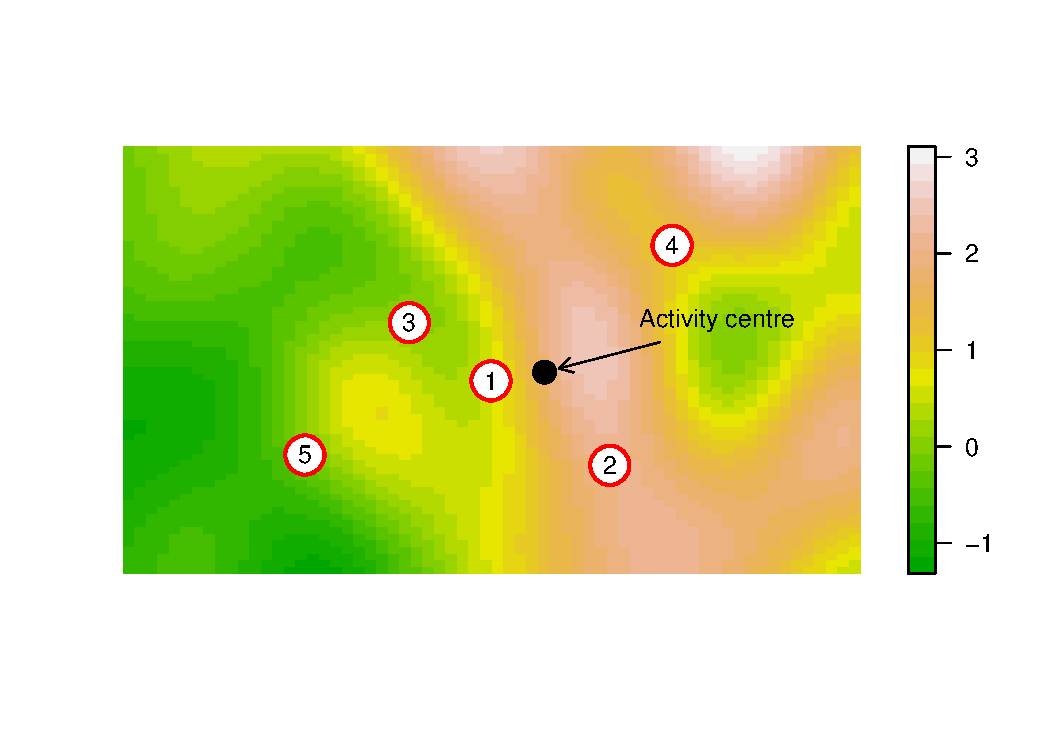
\includegraphics[width=12cm]{keepfigure/habitat.pdf}
\label{fig:ER+detfun_habitat}
\end{figure}

\begin{figure}[ht]
\caption{\small A plot showing an animal's average space usage over the survey period, expressed in terms of the number of times it is expected to encounter a detector at any point in the region during the survey. The locations of five detectors used on the survey are also shown.}
\centering
\vspace{-24pt}
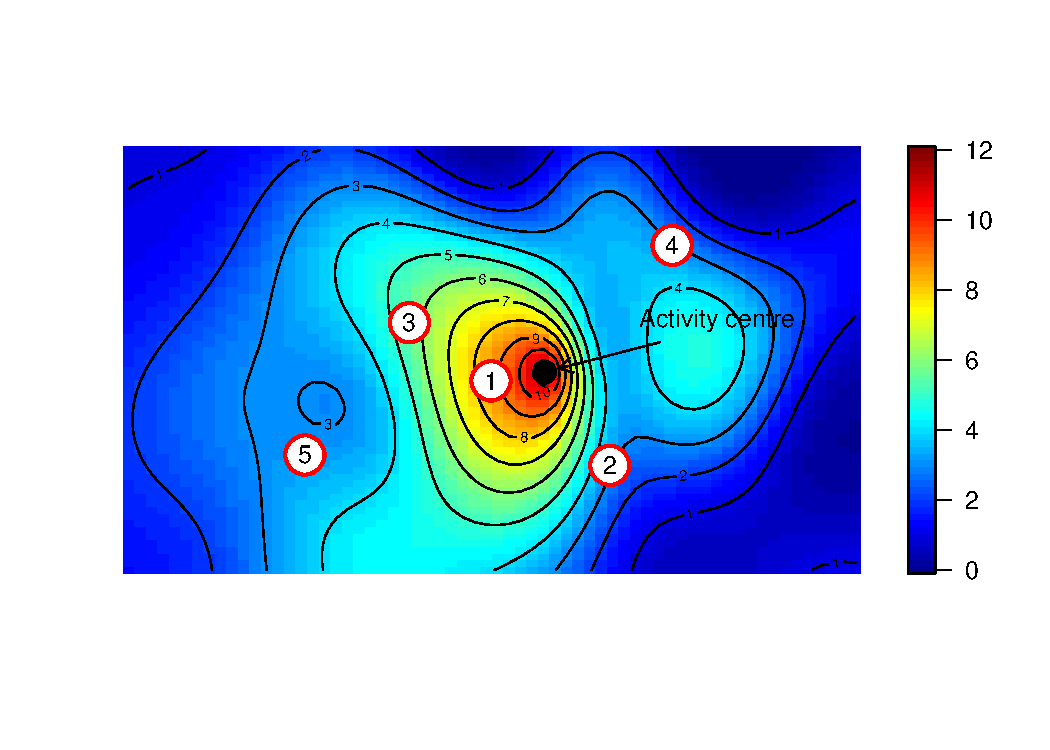
\includegraphics[width=12cm]{keepfigure/usage.pdf}
\label{fig:ER+detfun_habitat_encrate}
\end{figure}

We don't get to see maps like that in Figure~\ref{fig:ER+detfun_habitat_encrate} during a survey, all we see are the detections at each detector, and from these we try to reconstruct something like the figure, in addition to estimating animal density. In this chapter we focus on estimation the expected number of encounters as a function of distance from activity centre and leave density estimation aside until Chapter~\ref{sec:ch_spdetfn_integrating}. To keep things simple, we're initially going to (a) ignore habitat and consider expected encounter rate as a function of distance only and (b) work in one distance dimension rather than two. 

\subsection{Spatial capture histories and encounter functions}
\label{subsec:ER+detfun.spatialCH}

In one dimension, detectors are located at points along a line rather than points on a plane. Figure~\ref{fig:ER+detfun_enc} shows the five detectors of Figure~\ref{fig:ER+detfun_habitat_encrate} in one dimension, together with the number of times individual $i$ was detected at each detector. These data comprise a spatial capture history for individual $i$, which we can write as $\bm{\omega}_i=(n_{i1},n_{i2},n_{i3},n_{i4},n_{i5})=(11,5,2,1,0)$. Spatial capture histories like this (albeit with locations in two dimensions, not one) are all you get from a camera trap survey. Everything we estimate is based on these spatial capture histories.


\begin{figure}[ht]
\caption{\small Illustrative example of camera trap data in one dimension. The number of detections of individual $i$ on each of $j=1,\ldots,5$ cameras is shown, together with the location of each camera.}
\centering
\vspace{-24pt}
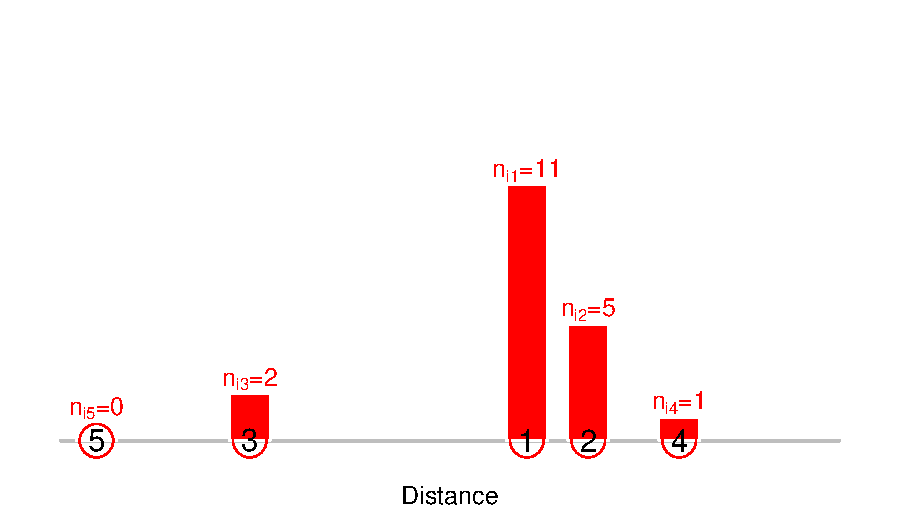
\includegraphics[width=10cm]{keepfigure/ObsN.pdf}
\label{fig:ER+detfun_enc}
\end{figure}

Although it is nothing like a map of expected encounters, Figure~\ref{fig:ER+detfun_enc} actually tells us quite a bit about the expected number of encounters of this individual at any point along the line. It tells us something about the location of the individual's activity centre: this is likely nearer detectors 1 and 2 than detector 3, because there were more encounters at 1 and 2 than at 3. The activity centre is likely between detectors 1 and 3, and closer to 1 than to 3. It suggests that the individual does not range as far as the distance from detector 1 to detector 5 (because we estimate that it is close to 1 and it had no encounters at detector 5). 

We can formalise these observations by fitting an encounter rate function to the spatial capture history data shown in Figure~\ref{fig:ER+detfun_enc}. To do this, let's assume that the encounter rate function has the shape of a Gaussian function, centred on an unknown activity centre at $\bm{s}_i$, with an unknown ``scale parameter'' $\sigma$ that determines the \todo[inline]{perhaps still vague}detector's range, and an unknown ``intercept'' $\lambda_0$ (the encounter rate of a detector placed at the activity centre). With these assumptions, the expected encounter rate at a point $\bm{x}_j$ that is a distance $d_{ij}=||\bm{s}_i-\bm{x}_j||$ from $\bm{s}_i$ is\todo[inline]{does this notation need definition?}

\be
\lambda(d_{ij})&=&\lambda_0\exp\left\{\frac{-d_{ij}^2}{2\sigma^2}\right\}.
\label{eq:ER+detfun.lambda.hn}
\ee

We can estimate $\lambda_0$ and $\sigma$ by fitting this function to the data in Figure~\ref{fig:ER+detfun_enc}. However, we need to take account of the survey duration to do this because the longer the survey, the higher the number of encounters will be. (Recall that $\lambda(d)$ is an encounter \textit{rate}, i.e. number of encounters \textit{per unit time}.) This is very easily done, because the expected number of encounters is proportional to the time spent surveying: if you survey for twice as long, you expect twice as many encounters. The expected \textit{number} of encounters on a survey of duration $T$ time units is just $\lambda(d)T$. This is shown in Figure~\ref{fig:ER+detfun_ENwithdists}.

\begin{figure}[ht]
\caption{\small The encounter rate function $\lambda(d)$ scaled by survey duration $T$ and centred at $\bm{s}_i$. Distances from $\bm{x}_i$ to each camera trap are shown below the curve and the expected number of encounters at each camera trap ($\lambda(d_{ij})T$ to camera trap $j=1,\ldots,5$) is marked on the curve.}
\centering
\vspace{-24pt}
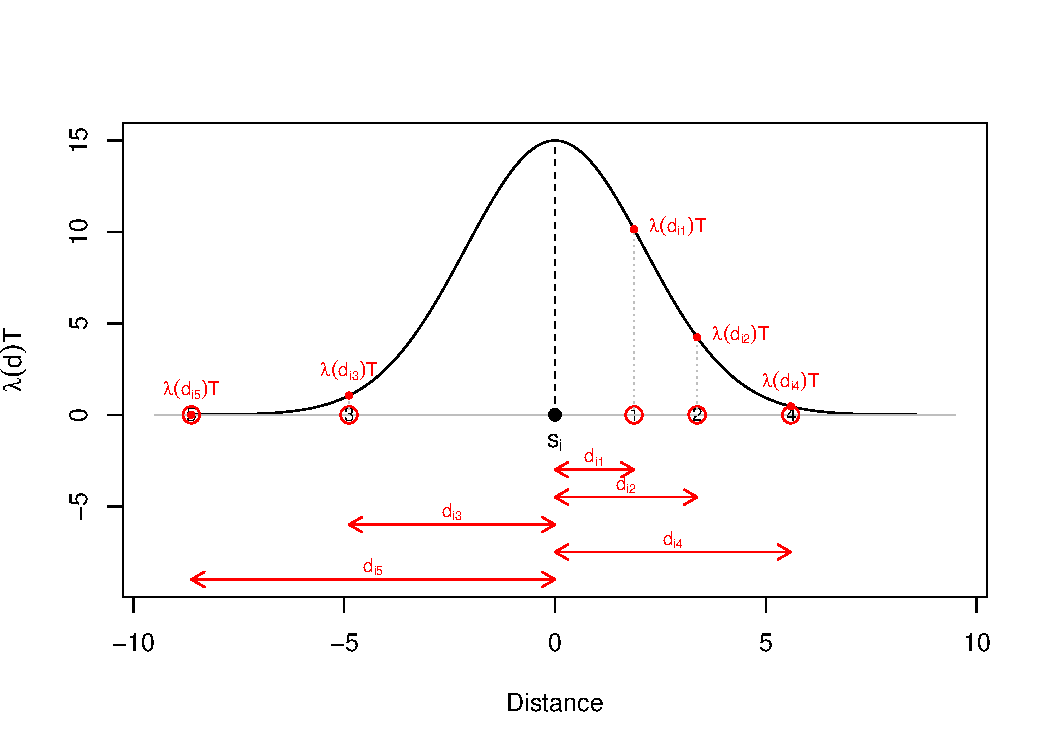
\includegraphics[width=11cm]{keepfigure/ENwithdists.pdf}
\label{fig:ER+detfun_ENwithdists}
\end{figure}

If we fit this function to the observed numbers of encounters shown in Figure~\ref{fig:ER+detfun_enc}, we get Figure~\ref{fig:ER+detfun_ENwithdists}. In summary, given the locations of detectors and an expected encounter rate model with unknown intercept and range, we can use spatial capture histories to estimate the expected number of encounters of individuals at any distance from their activity centres. This also allows us to estimate the probability of detecting an individual at all, because the probability of detection is just the probability of getting more than zero encounters -- see Section~\ref{sec:ER+detfun.binary}

We use exactly the same methods to estimate encounter rate functions in two dimensions. In fact, because the distance measure used in the one-dimensional example above was the two-dimensional distance from the activity centre to the detectors, this example was actually two-dimensional - its just that we plotted the encounter function in the distance dimension rather than on the plane.

\subsection{The capture history likelihood component: count data}
\label{subsec:ER+detfun.ERlikelihood}

The encounter rate model $\lambda(d)$ on its own is not enough to fit it to the observed capture history. An appropriate model also needs to explain why the observed number of encounters differs from the expected number. The model needs a random component. 

Whenever events occur independently at some fixed average rate ($\lambda(d)$ in our case), the number of events (encounters in our case) occurring over a time period $T$ has a Poisson distribution with parameter $\lambda(d)T$. \todo[inline]{awkward sentence structure} Our model for the observed number of encounters (under the assumption that encounters are independent events) is if individual $i$'s activity centre is a distance $d_{ij}$ from detector $j$ then $n_{ij}$, the number of encounters of individual $i$ with detector $j$ in a time period $T$, is a Poisson random variable with parameter $\lambda(d_{ij})T$. We write this as
\be
[n_{ij}|\bm{s}_i]&=&\mbox{Po}\left(n_{ij};\lambda(d_{ij})T\right).
\ee
\noindent
(Note that we need the activity centre $\bm{s}_i$ to be known to know $d_{ij}$.)

Assuming that detections occur independently at each of $J$ detectors (as might be reasonable for camera trap surveys, or acoustic surveys), the capture history for individual $i$ is distributed as the product of independent Poisson random variables:
\be
[\bm{\omega}_i|\bm{s}_i]&=&\prod_{j=1}^J\mbox{Po}\left(n_{ij};\lambda(d_{ij})T\right).
\ee

And if encounters by different individuals with detectors are also independent then the set of $n$ observed capture histories $\bm{\Omega}_n=(\bm{\omega}_1,\ldots,\bm{\omega}_n)$, given the activity centres $\bm{S}_n=(\bm{s}_1,\ldots,\bm{s}_n)$ of all $n$ detected individuals, is also distributed as the product of independent Poisson random variables, and constitutes 
\begin{svgraybox}
\bf{The capture history likelihood component for count data}
\be
[\bm{\Omega}_n|\bm{S}_n]&=&\prod_{i=1}^n\prod_{j=1}^J\mbox{Po}\left(n_{ij};\lambda(d_{ij})T\right)
\label{eq:ER+detfun.P.Omega.count}
\ee
\end{svgraybox}

This is the probability of observing capture histories $\bm{\omega}_1,\ldots,\bm{\omega}_n$ for individuals $i=1,\ldots,n$, given that the $i$th individual's activity centre is at distances $d_{i1},\ldots,d_{iJ}$ from detectors $j=1,\ldots,J$. 

\section{A simple spatial binary detection model}
\label{sec:ER+detfun.simple.det.model}

In the above example, which is appropriate for detectors like camera traps or acoustic arrays, the capture history consisted of the number of encounters at each detector. But not all kinds of detectors generate this kind of capture history. Suppose  you performed a survey with hair snares rather than camera traps or microphones.

With hair snares you can't tell how often individuals encountered detectors, only whether or not they did encounter them (whether or not there is at least one identifiable hair in the snare). In this case, using 1 to denote encounter and 0 to denote no encounter, the capture history from the example above would be $(1,1,1,1,0)$ instead of $(11,5,2,1,0)$. Nevertheless, the Poisson encounter rate model is still applicable, because the probability that individual $i$ encountered detector $j$ is just the probability that $n_{ij}$ is greater than zero, i.e.
\be
\mathbb{P}(n_{ij}>0)&=&1-\mathbb{P}(n_{ij}=0)
\;=\;1-e^{-\lambda(d_{ij})T}. 
\ee
We can write the probability that individual $i$ is detected by (i.e. encounters) detector $j$ as 
\be
p(d_{ij},T)&=&1-e^{-\lambda(d_{ij})T}. 
\label{eq:ER+detfun.binaryp}
\ee
Notice that this probability depends on the survey duration, $T$. If the same detector is used for different periods of time on two occasions, it will have different detection probabilities on the two occasions, and if identical detectors are used for different periods of time on the same occasion, they will have different detection probabilities. It is important to take account of this when doing SCR inference.


\begin{figure}[ht]
\caption{\small The time-scaled encounter rate function $\lambda(d)T$ fitted to the data in Figure~\ref{fig:ER+detfun_enc}. The black dot is the estimated activity centre location.}
\centering
\vspace{-24pt}
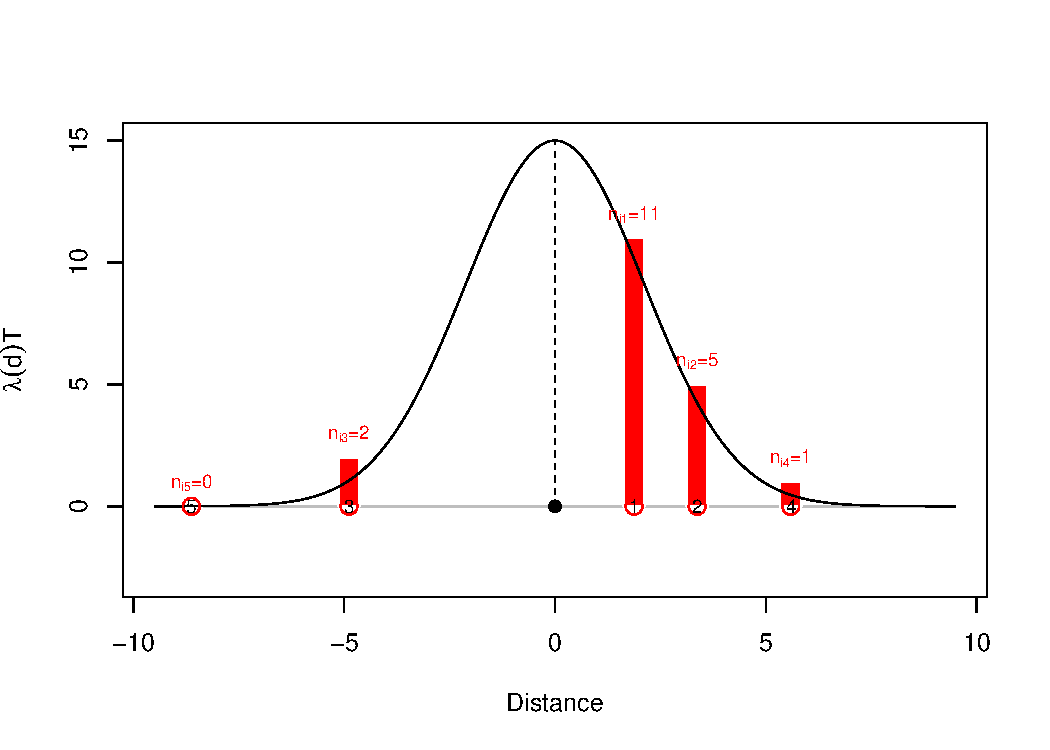
\includegraphics[width=11cm]{keepfigure/EandN.pdf}
\label{fig:ER+detfun_EandN}
\end{figure}

%\afterpage{\clearpage}

The binary detection function $p(d_{ij},T)$ for the encounter rate model $\lambda(d_{ij})$ shown in Figure~\ref{fig:ER+detfun_EandN} is shown in Figure~\ref{fig:ER+detfun_binp}. Notice that while the encounter rate model was specified to have a Gaussian function shape (see Eqn~\eqref{eq:ER+detfun.lambda.hn} and Figure~\ref{fig:ER+detfun_EandN}), this leads to a detection function $p(d_{ij},T)$ that does not have a Gaussian function shape (see Eqn~\eqref{eq:ER+detfun.binaryp} and Figure~\ref{fig:ER+detfun_binp}). Conversely, if we specify that the detection function $p(d_{ij},T)$ has a Gaussian function shape, then the corresponding encounter rate function would not have a Gaussian function shape.

\begin{figure}[ht]
\caption{\small The detection probability function (black curve) corresponding to the encounter function shown in Figure~\ref{fig:ER+detfun_EandN}, with binary capture history given by the bars and the binary data below the $x$-axis.}
\centering
\vspace{-24pt}
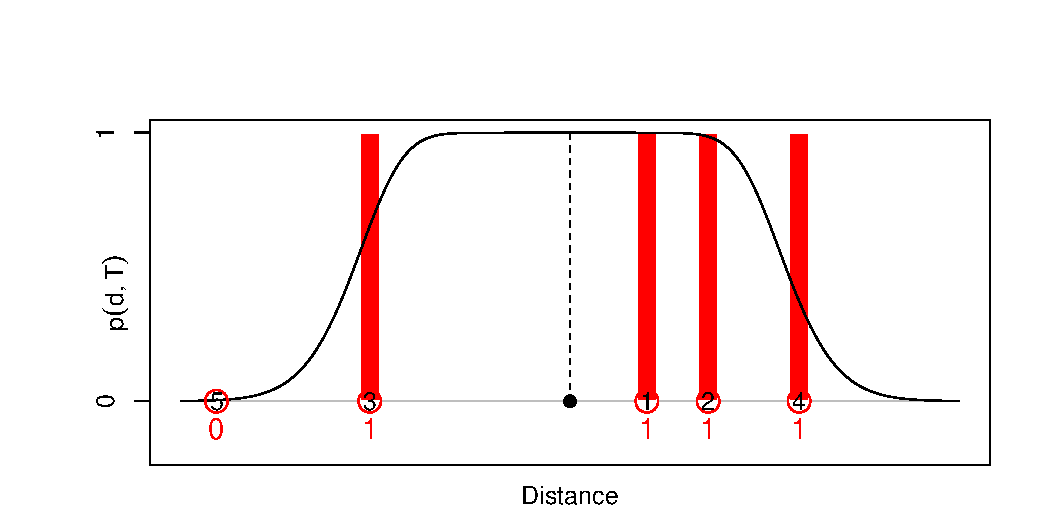
\includegraphics[width=11cm]{keepfigure/binp.pdf}
\label{fig:ER+detfun_binp}
\end{figure}


\subsection{The capture history likelihood component: binary data}
\label{subsec:ER+detfun.binarylikelihood}

Using $\delta_{ij}$ to indicate whether or not individual $i$ encountered detector $j$ ($\delta_{ij}=1$ if detected, $\delta_{ij}=0$ if not), we can write the capture history as $\bm{\omega}_i=(\delta_{i1},\ldots,\delta_{iJ})$. Assuming that encounters occur independently on each detector, then an individual's capture history is distributed as the product of Bernoulli random variable with ``success'' probabilities $p(d_{ij},T)$ ($j=1,\ldots,J$), and we write
\be
[\bm{\omega}_i|\bm{s}_i]&=&\prod_{j=1}^J\mbox{Bern}\left(\delta_{ij};p(d_{ij},T)\right).
\ee

If encounters by different individuals are also independent then the set of $n$ observed capture histories $\bm{\Omega}_n=(\bm{\omega}_1,\ldots,\bm{\omega}_n)$ is  distributed as the product of independent Bernoulli random variables:
\begin{svgraybox}
\bf{The capture history likelihood component for independent binary data}
\be
[\bm{\Omega}_n|\bm{S}_n]&=&\prod_{i=1}^n\prod_{j=1}^J\mbox{Bern}\left(\delta_{ij};p(d_{ij},T)\right)
\label{eq:ER+detfun.P.Omega.binary}
\ee
\end{svgraybox}

\section{Should you model $p(d,T)$ or $\lambda(d)$?}

It doesn't matter. You can model either. Eqn~\eqref{eq:ER+detfun.binaryp} gives us a way of converting between encounter rate $\lambda(d)$ and detection probability $p(d,T)$:
\be
p(d,T)&=&1-e^{-\lambda(d)T} 
\label{eq:ER+detfun.lambda.to.p}
\ee
\noindent
or making $\lambda(d)$ the subject of the equation:
\be
\lambda(d)&=&\frac{-\log\left\{1-p(d,T)\right\}}{T}.
\label{eq:ER+detfun.p.to.lambda}
\ee
If you have hair snare data, and choose to specify a model for $\lambda(d)$ (e.g. specify that it is has a Gaussian function shape), then given the survey duration $T$, this is easily converted into a model for $p(d,T)$ using Eqn~\eqref{eq:ER+detfun.lambda.to.p}. If you have camera trap data, you can choose to specify a model for $p(d,T)$ for a given $T$ (e.g. specify that it is has a Gaussian function shape for this $T$), and this is easily converted into an encounter rate model $\lambda(d)$ using Eqn~\eqref{eq:ER+detfun.p.to.lambda}.

For example if you specified that when $T=1$, $p(d,T)$ has a Gaussian shape with intercept parameter $g_0$ (the probability of detection when the activity centre is at the detector) and range parameter $\sigma$:
\be
p(d,T=1)&=&g_0\exp\left\{\frac{-d^2}{2\sigma^2}\right\}.
\label{eq:ER+detfun.p.hn}
\ee
\noindent
then the corresponding $\lambda(d)$ is
\be
\lambda(d)&=&\frac{-\log\left\{1-p(d,T=1)\right\}}{1}
\;=\;-\log\left\{1-g_0\exp\left\{\frac{-d^2}{2\sigma^2}\right\}\right\}
\label{eq:ER+detfun.Guassian.p.to.lambda}
\ee

Note, however, that if $p(d,T)$ has some specific shape (Gaussian, for example) for a survey duration $T$, it will \textit{not} have this shape for any other $T$. If you specify that $p(d,T)$ has a Gaussian shape for your default survey duration and then some detectors fail halfway through the survey, these detectors will not have a Gaussian detection function shape. This is usually not a big deal because (a) unless $T$ changes a lot, the shapes will not be very different and (b) you never know the true shape of $p(d,T)$ for any $T$ anyway. But it is as well to be aware of that the shape of $p(d,T)$ depends on $T$.

We usually have very little idea what the detection or encounter rate function shape should be. We have a range of functional forms for each and choosing between them is a model selection question. Whether it is better to specify a form for $p(d,T)$ or for $\lambda(d)$ is also a model selection question. 


\section{Count and binary data application}
\label{sec:ER+detfun.count+binary.eg}

To illustrate the application of the above ideas, we will use the package \texttt{secr} to fit simple models to count data from a camera trap survey of leopards in the Kruger National Park, and to a binary version of these data.
\todo[inline]{Need to introduce this dataset in the introduction (?), and acknowledge source.}

Here we focus on the expected encounter rate function and detection function specification. To fit an SCR model you also need to specify (a) a model for activity centre density and distribution and (b) because activity centres are unobserved, you need to specify a region within which the activity centres of the detected individuals could be, and outside of which they could not be. For (a) will use the default density model here, which assumes unknown but equal density of activity centres everywhere, and we will use a prepared ``mask'' (an \texttt{secr} term) that specifies the region (b). Density models are dealt with in detail in Chapter~\ref{ch:SPmod} and masks are explained further in Section~\ref{sec:??}.

The necessary data and associated fitted objects are obtained by loading the library \texttt{scrmlebook} package and getting the data and other \texttt{R} objects for this chapter, as follows:
{\small
\begin{knitrout}
\definecolor{shadecolor}{rgb}{0.969, 0.969, 0.969}\color{fgcolor}\begin{kframe}
\begin{alltt}
\hlkwd{library}\hlstd{(scrmlebook)}
\hlkwd{data}\hlstd{(}\hlstr{"ERdetfun-data"}\hlstd{)}
\hlkwd{data}\hlstd{(}\hlstr{"ERdetfun-fits"}\hlstd{)}
\end{alltt}
\end{kframe}
\end{knitrout}
}

The first \texttt{data} command loads the count capture history in \texttt{R} object \texttt{kruger.capt}, the corresponding binary capture history in \texttt{kruger.capt.bin} and the mask object in \texttt{kruger.mask}. The second loads all the models that are fitted in this chapter (the code some of which is given below). These are all objects that were created using the \texttt{secr} library. Details of the data and the fits can be viewed in the \texttt{scrmlebook} help files as follows
{\small
\begin{knitrout}
\definecolor{shadecolor}{rgb}{0.969, 0.969, 0.969}\color{fgcolor}\begin{kframe}
\begin{alltt}
\hlkwd{help}\hlstd{(}\hlstr{"ERdetfun-data"}\hlstd{)}
\hlkwd{help}\hlstd{(}\hlstr{"ERdetfun-fits"}\hlstd{)}
\end{alltt}
\end{kframe}
\end{knitrout}
}

\subsection{Example fits to count data}

To specify an encounter rate model we need to specify the functional form to use and to say how its parameters depend on covariates. We postpone consideration of covariates until later and so use the syntax \url{~}\texttt{1}, which indicates no dependence on covariates.

In \texttt{secr}-speak a model with Gaussian shape is called a ``half-normal'' model (a name derived from the distance sampling literature \todo{insert citation?}), and encounter rate functions are called ``hazard'' functions (a name that derives from survival analysis literature). Specifying that the model is ``\texttt{HHN}'' in \texttt{secr}-speak, is specifying that it is an encounter rate model (the first \texttt{H} is for ``hazard'') with half-normal shape (``\texttt{HN}''). As \texttt{secr}-speak for $\lambda_0$ and $\sigma$ is ``\texttt{lambda0}'' and ``\texttt{sigma}'', the specification for an encounter rate model with Gaussian shape is as shown below.

We fit this model using the \texttt{secr} function \texttt{secr.fit}, by passing the function the capture history object \texttt{kruger.fit} (which contains in it details of detector locations), the model specification in the form of \texttt{er.model} and \texttt{detfn} below, and information on the region that could contain the activity centres of detected individuals (\texttt{kruger.mask}).

{\small
\begin{knitrout}
\definecolor{shadecolor}{rgb}{0.969, 0.969, 0.969}\color{fgcolor}\begin{kframe}
\begin{alltt}
\hlstd{er.hn.fit} \hlkwb{<-} \hlkwd{secr.fit}\hlstd{(kruger.capt,} \hlkwc{mask}\hlstd{=kruger.mask,}
                      \hlkwc{model}\hlstd{=}\hlkwd{list}\hlstd{(lambda0}\hlopt{~}\hlnum{1}\hlstd{,sigma}\hlopt{~}\hlnum{1}\hlstd{),} \hlkwc{detectfn}\hlstd{=}\hlstr{"HHN"}\hlstd{)}
\end{alltt}
\end{kframe}
\end{knitrout}
}


We will also fit an encounter rate model with ``hazard rate'' shape. \todo[inline]{move out of this application section}This is defined as follows
\be
\lambda(d)&=&\lambda_0\left(1-\exp\left\{-\left[\frac{d}{\sigma}\right]^{-b}\right\}\right).
\ee
\noindent 
It has one more parameter ($b$) than a Gaussian model and is hence more flexible. Its shape can be seen in Figure~\ref{fig:ERdetfun.hrfit}. 

An encounter rate model with hazard rate shape is called ``\texttt{HHR}'' in \texttt{secr}-speak, and we can fit it as follows:
{\small
\begin{knitrout}
\definecolor{shadecolor}{rgb}{0.969, 0.969, 0.969}\color{fgcolor}\begin{kframe}
\begin{alltt}
\hlstd{er.hr.fit} \hlkwb{<-} \hlkwd{secr.fit}\hlstd{(kruger.capt,} \hlkwc{mask}\hlstd{=kruger.mask,}
                      \hlkwc{model}\hlstd{=}\hlkwd{list}\hlstd{(lambda0}\hlopt{~}\hlnum{1}\hlstd{,sigma}\hlopt{~}\hlnum{1}\hlstd{),} \hlkwc{detectfn}\hlstd{=}\hlstr{"HHR"}\hlstd{)}
\end{alltt}
\end{kframe}
\end{knitrout}
}

The Gaussian and hazard models can be compared on the basis of AIC$_c$ as follows
{\small
% latex table generated in R 3.2.3 by xtable 1.8-2 package
% Sun Oct 16 14:58:13 2016
\begin{table}[ht]
\centering
\begin{tabular}{rllrr}
  \hline
 & model & detectfn & dAICc & AICcwt \\ 
  \hline
er.hr.fit & D\~{}1 lambda0\~{}1 sigma\~{}1 z\~{}1 & hazard hazard rate & 0.00 & 0.67 \\ 
  er.hn.fit & D\~{}1 lambda0\~{}1 sigma\~{}1 & hazard halfnormal & 1.45 & 0.33 \\ 
   \hline
\end{tabular}
\caption{Model selection criteria for hazard rate and Gaussian encounter rate models fitted to Kruger count data.} 
\label{tab:ERdetfun.countmodsel}
\end{table}

}

\noindent
With a $\Delta$AIC$_c$ of only about 1.45 (Table~\ref{tab:ERdetfun.countmodsel}), this suggests that the hazard rate model is slightly better than the Gaussian model. Point estimates and upper and lower 95\% confidence interval bounds for density, $\lambda_0$, $\sigma$ and the hazard rate parameter $b$ (called \texttt{z} in \texttt{secr}-speak) are show in Table~\ref{tab:ERdetfun.countests}.

{\small
% latex table generated in R 3.2.3 by xtable 1.8-2 package
% Sun Oct 16 14:58:13 2016
\begin{table}[ht]
\centering
\begin{tabular}{rrrr}
  \hline
 & estimate & lcl & ucl \\ 
  \hline
D & 0.0002 & 0.0001 & 0.0003 \\ 
  lambda0 & 1.9105 & 0.5875 & 6.2124 \\ 
  sigma & 1262.7018 & 503.2888 & 3167.9935 \\ 
  z & 2.1126 & 1.6540 & 2.6984 \\ 
   \hline
\end{tabular}
\caption{Parameter estimates and 95\% confidence bounds for density, $\lambda_0$ and hazard rate parameter $b$.} 
\label{tab:ERdetfun.countests}
\end{table}

} 


A plot similar to Figure~\ref{fig:ER+detfun_EandN} would show how the capture frequencies have informed the encounter rate model, as explained above. However, because we have 62 detectors here rather than just 5, a plot like Figure~\ref{fig:ER+detfun_EandN} is too messy to be useful. Instead of using exact distances to detectors, we will use distance intervals and count the average number of detections for all detectors in each distance interval. Because we are operating in two spatial dimensions, negative and positive distances are not well defined, so we will do a plot only on positive distances (as if the negative distances had been folded over onto the positive ones). Doing this with the \texttt{scrmlebook} library function \texttt{plot.er.fit}, we get Figure~\ref{fig:ERdetfun.hrfit}. 

{\small
\begin{knitrout}
\definecolor{shadecolor}{rgb}{0.969, 0.969, 0.969}\color{fgcolor}\begin{kframe}
\begin{alltt}
\hlkwd{plot.er.fit}\hlstd{(er.hr.fit,}\hlkwc{dmax}\hlstd{=}\hlnum{15000}\hlstd{,}\hlkwc{binwidth}\hlstd{=}\hlnum{1000}\hlstd{,}\hlkwc{lwd}\hlstd{=}\hlnum{3}\hlstd{,}
            \hlkwc{xlab}\hlstd{=}\hlstr{"Distance, d (m)"}\hlstd{,}\hlkwc{ylab}\hlstd{=}\hlkwd{expression}\hlstd{(}\hlkwd{hat}\hlstd{(lambda)(d)))}
\hlkwd{plot}\hlstd{(er.hn.fit,}\hlkwc{xval}\hlstd{=}\hlkwd{seq}\hlstd{(}\hlnum{0}\hlstd{,}\hlnum{15000}\hlstd{,}\hlkwc{length}\hlstd{=}\hlnum{200}\hlstd{),}\hlkwc{lwd}\hlstd{=}\hlnum{3}\hlstd{,}\hlkwc{add}\hlstd{=}\hlnum{TRUE}\hlstd{,}\hlkwc{col}\hlstd{=}\hlstr{"gray"}\hlstd{)}
\hlkwd{legend}\hlstd{(}\hlstr{"top"}\hlstd{,}\hlkwc{legend}\hlstd{=}\hlkwd{c}\hlstd{(}\hlstr{"Gaussian (or half-normal)"}\hlstd{,}\hlstr{"Hazard rate"}\hlstd{),}
       \hlkwc{col}\hlstd{=}\hlkwd{c}\hlstd{(}\hlstr{"gray"}\hlstd{,}\hlstr{"black"}\hlstd{),}\hlkwc{lwd}\hlstd{=}\hlnum{3}\hlstd{,}\hlkwc{bty}\hlstd{=}\hlstr{"n"}\hlstd{,}\hlkwc{cex}\hlstd{=}\hlnum{0.8}\hlstd{)}
\end{alltt}
\end{kframe}
\end{knitrout}
} 


\begin{figure}[ht]
\caption{\small Histogram of average number of detections per detector against distance of detectors from estimated activity centre locations, by 3,000m distance interval. The estimated Gaussian and hazard-rate encounter rate models are plotted over the histogram.}
\centering
\vspace{-24pt}
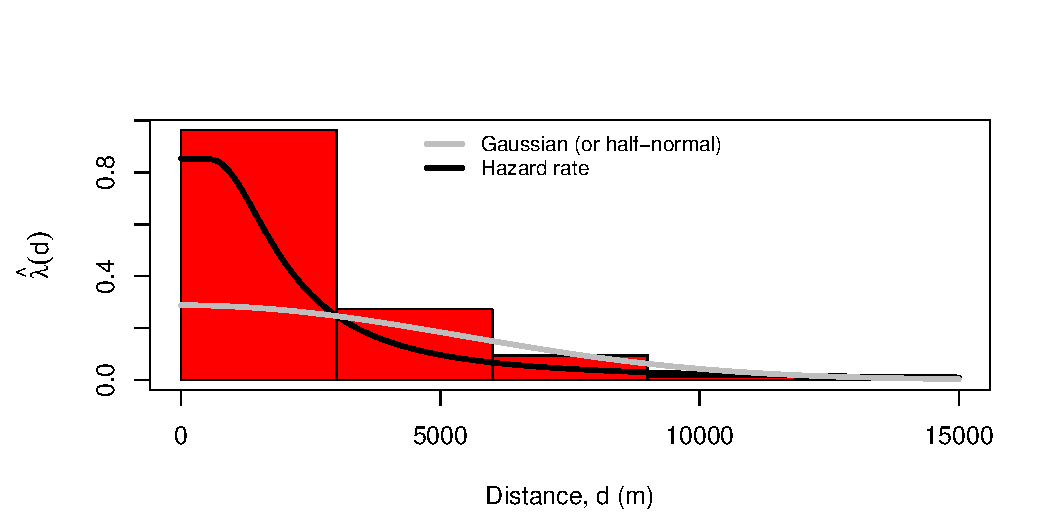
\includegraphics[width=11cm]{keepfigure/ERdetfun-hrfit.pdf}
\label{fig:ERdetfun.hrfit}
\end{figure}

The Gaussian model seems to be a  poor fit to the average encounter data, and in this plot looks a  worse fit than the hazard rate model. However, we need to be cautious about over-interpreting this figure because it is based on the \textit{estimated} locations of activity centres, and these have substantial uncertainty associated with them, as shown in Figure~\ref{fig:ERdetfun-locest}. This uncertainty is not incorporated into Figure~\ref{fig:ERdetfun.hrfit}. We can't really conclude a lot more from this plot than that the encounter rate does decline with distance, as expected, and that animals were very unlikely to venture more than about 15km from their activity centres over the survey period.

\begin{figure}[ht]
\caption{\small Kruger leopard study camera traps (black dots) and estimated \todo[inline]{contours will need more explanation}probability contours of the activity centres of 5 detected individuals. (The average distance between the cameras is 3264m.)}
\centering
\vspace{-24pt}
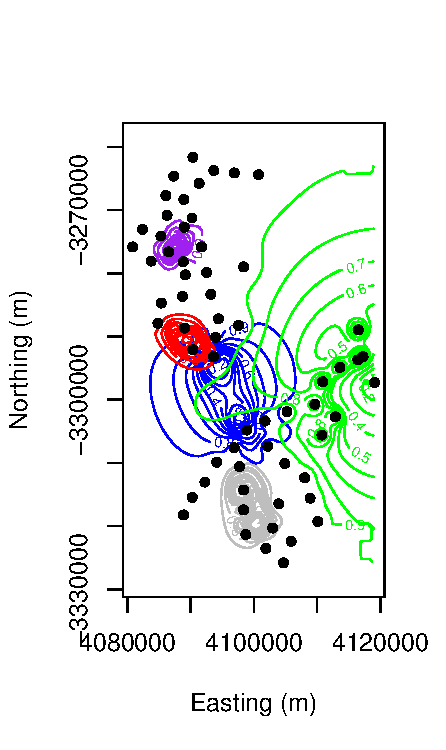
\includegraphics[width=6cm]{keepfigure/ERdetfun-locest.pdf}
\label{fig:ERdetfun-locest}
\end{figure}

\todo[inline]{beginning of interpretation section--subsection?}
Interestingly, \todo[inline]{but density isn't reported here, should it be discussed?}the estimated leopard density from the hazard rate model is only about 5\% smaller than that from the Gaussian model, despite their very different shapes (Figure~\ref{fig:ERdetfun.hrfit}). This is a fairly typical feature of SCR models: different models can give quite different encounter rate (or detection function) shapes but very similar density estimates. The root cause of this is that  we have rather poor information on the distances of detectors from activity centres because we do not observe the activity centres, and as a result there is relatively little information in the data to tell us about the shape of the encounter rate function or detection function. There is usually quite good information on \textit{area under the encounter rate or detection function}. In our case the areas under the Gaussian and hazard rate curves differ by only 6\%. 

A moral of this story is ``Be careful not to over-interpret encounter rate or detection functions.''.

We could also specify Gaussian or hazard-rate forms for the detection function rather than the encounter rate function. For example, a detection function with hazard rate form is fitted thus:
{\small
\begin{knitrout}
\definecolor{shadecolor}{rgb}{0.969, 0.969, 0.969}\color{fgcolor}\begin{kframe}
\begin{alltt}
\hlstd{df.hr.fit} \hlkwb{<-} \hlkwd{secr.fit}\hlstd{(kruger.capt,} \hlkwc{mask}\hlstd{=kruger.mask,}
                      \hlkwc{model}\hlstd{=}\hlkwd{list}\hlstd{(lambda0}\hlopt{~}\hlnum{1}\hlstd{,sigma}\hlopt{~}\hlnum{1}\hlstd{),} \hlkwc{detectfn}\hlstd{=}\hlstr{"HR"}\hlstd{)}
\end{alltt}
\end{kframe}
\end{knitrout}
}
Note that this detection function applies over the duration of the survey. We are implicitly saying that $T=1$ for the duration of the survey, i.e., that time units are ``this-survey-length''. Specifying the same detection function for a survey of a different length would be inconsistent.

\todo[inline]{not all models in table shown in text...}Having fitted models with both Gaussian and hazard-rate forms for the encounter rate function and the detection function, we can compare models using AIC$_c$ again:
\todo[inline]{Tables 1.3 and 1.4 not referenced in text.}

{\small
% latex table generated in R 3.2.3 by xtable 1.8-2 package
% Sun Oct 16 14:58:14 2016
\begin{table}[ht]
\centering
\begin{tabular}{rllrr}
  \hline
 & model & detectfn & dAICc & AICcwt \\ 
  \hline
er.hr.fit & D\~{}1 lambda0\~{}1 sigma\~{}1 z\~{}1 & hazard hazard rate & 0.00 & 0.34 \\ 
  df.hr.fit & D\~{}1 g0\~{}1 sigma\~{}1 z\~{}1 & hazard rate & 0.12 & 0.32 \\ 
  df.hn.fit & D\~{}1 g0\~{}1 sigma\~{}1 & halfnormal & 1.25 & 0.18 \\ 
  er.hn.fit & D\~{}1 lambda0\~{}1 sigma\~{}1 & hazard halfnormal & 1.45 & 0.16 \\ 
   \hline
\end{tabular}
\caption{Model selection criteria for hazard rate and Gaussian detection function models fitted to Kruger count data.} 
\label{tab:ERdetfun.detfn.countmodsel}
\end{table}

}
\noindent
It is apparent from this that it makes very little difference whether you specify the shape of the encounter rate function or the shape of the detection function. The main difference is that the shape of the encounter rate function is independent of the survey duration, whereas the shape of the detection function changes with survey length. This makes the encounter rate function a ``common currency'' for all survey durations.

\subsection{Example fits to binary data}

Here we suppose that instead of camera-traps, the detectors on the Kruger leopard survey were hair snares (and that identification was by way of DNA). This leads to some loss of information because instead of counts we get only binary detected/undetected data at each detector.

We can fit models to these binary capture history data (in \texttt{kruger.capt.bin}) much as we did with the count data, but having specified that detector are what \texttt{secr} calls ``proximity'' detectors when we created the capture history object. You can see what kind of detectors are in a capture history object thus:
{\small
\begin{knitrout}
\definecolor{shadecolor}{rgb}{0.969, 0.969, 0.969}\color{fgcolor}\begin{kframe}
\begin{alltt}
\hlkwd{detector}\hlstd{(kruger.cams)}
\end{alltt}
\begin{verbatim}
## [1] "count"
\end{verbatim}
\begin{alltt}
\hlkwd{detector}\hlstd{(kruger.cams.bin)}
\end{alltt}
\begin{verbatim}
## [1] "proximity"
\end{verbatim}
\end{kframe}
\end{knitrout}
} 

Here is code to fit an encounter rate function model with hazard rate form to the binary data, for example:
{\small
\begin{knitrout}
\definecolor{shadecolor}{rgb}{0.969, 0.969, 0.969}\color{fgcolor}\begin{kframe}
\begin{alltt}
\hlstd{er.bin.hn.fit} \hlkwb{<-} \hlkwd{secr.fit}\hlstd{(kruger.capt.bin,} \hlkwc{mask}\hlstd{=kruger.mask,}
                          \hlkwc{model}\hlstd{=}\hlkwd{list}\hlstd{(g0}\hlopt{~}\hlnum{1}\hlstd{,sigma}\hlopt{~}\hlnum{1}\hlstd{),} \hlkwc{detectfn}\hlstd{=}\hlstr{"HHN"}\hlstd{)}
\end{alltt}
\end{kframe}
\end{knitrout}
} 

And to compare various models fitted to these binary data:
{\small
% latex table generated in R 3.2.3 by xtable 1.8-2 package
% Sun Oct 16 14:58:14 2016
\begin{table}[ht]
\centering
\begin{tabular}{rllrr}
  \hline
 & model & detectfn & dAICc & AICcwt \\ 
  \hline
df.bin.hn.fit & D\~{}1 g0\~{}1 sigma\~{}1 & halfnormal & 0.00 & 0.28 \\ 
  er.bin.hn.fit & D\~{}1 lambda0\~{}1 sigma\~{}1 & hazard halfnormal & 0.02 & 0.28 \\ 
  df.bin.hr.fit & D\~{}1 g0\~{}1 sigma\~{}1 z\~{}1 & hazard rate & 0.53 & 0.22 \\ 
  er.bin.hr.fit & D\~{}1 lambda0\~{}1 sigma\~{}1 z\~{}1 & hazard hazard rate & 0.56 & 0.21 \\ 
   \hline
\end{tabular}
\caption{Model selection criteria for hazard rate and Gaussian detection function models fitted to Kruger binary data.} 
\label{tab:ERdetfun.detfn.binarymodsel}
\end{table}

}


 %DLB


\section{Occasions: recaptures across space and time}
\label{sec:ER+detfun.occasions}

A notable feature of the example above was that the word ``occasion'' was not used. This might be surprising to you if you have a capture-recapture (CR) background since occasions are absolutely central to conventional (non-spatial) CR. In non-spatial CR, recaptures occur on different occasions in time and you can't get recaptures unless you have occasions. This is not true of SCR, where you can get \textit{recaptures over space} rather than, or in addition to, recaptures over time.

Instead of detections (or not) on each of a number of occasions in \textit{time}, we had detections (or not) at each of a number detectors in \textit{space} in the example above. This allowed us to estimate the expected number of encounters (and hence detection probability, since detection is just at least one encounter) when we have only a single sampling occasion. But you can't do this if your detectors are traps that hold animals when they detect them. 

We delay dealing with such traps until Chapter~\ref{ch:detector types}. But here we extend the above models to include occasions, which we index by $k=1,\ldots,K$. The count and binary likelihood functions of Eqns~\eqref{eq:ER+detfun.P.Omega.count} and \eqref{eq:ER+detfun.P.Omega.binary} are easily extended to include multiple occasions like this:
\begin{svgraybox}
\bf{The capture history likelihood component for count data (multi-occasion)}
\be
[\bm{\Omega}_n|\bm{S}_n]&=&\prod_{i=1}^n\prod_{j=1}^J\prod_{k=1}^K\mbox{Po}\left(n_{ijk};\lambda(d_{ijk})T_k\right)
\label{eq:ER+detfun.P.Omega.count.occ}
\ee
\end{svgraybox}
and this:
\begin{svgraybox}
\bf{The capture history likelihood component for independent binary data (multi-occasion)}
\be
[\bm{\Omega}_n|\bm{S}_n]&=&\prod_{i=1}^n\prod_{j=1}^J\prod_{k=1}^K\mbox{Bern}\left(\delta_{ijk};p(d_{ijk},T_k)\right)
\label{eq:ER+detfun.P.Omega.binary.occ}
\ee
\end{svgraybox}
\noindent
where
\begin{svgraybox}
\bd
\item[$n_{ijk}$] is the number of detections of individual $i$ at detector $j$ on occasion $k$,
\item[$\delta_{ijk}$] is 1 if individual $i$ was detected at detector $j$ on occasion $k$,
\item[$d_{ijk}$] is the distance of the activity centre of individual $i$ from detector $j$ on occasion $k$. Note that this is a latent variable - we do not observe it.
\item[$T_k$] is the duration of the $k$th occasion.
\ed
\end{svgraybox}

\section{Strata: no recaptures across space and time}
\label{sec:ER+detfun.strata}

It is sometimes useful to analyse multiple survey units that might share common encounter rate or detection function parameters, but between which recaptures cannot occur. These might be distinct spatial units (regions separated by larger distances than individuals would travel over the survey period, for example), or they might be surveys of the same region at times that are so far apart that no marks from one occasion are identifiable on other occasions. In survey parlance these are commonly called ``strata''. In \texttt{secr}-speak they are ``sessions''. (\cite{Royle+al:14} use both ``session'' and ``occasion'' to refer to what we call ``occasion'' in this book.)

In this case, each stratum is like a separate mini-survey that could be analysed on its own, without the other strata. But if some parameters may be shared across strata (if they might have a common $\sigma$, for example), then the analysis must combine the strata. Because no recaptures (as opposed to parameters) are shared across strata, the capture histories are independent between strata and the corresponding multi-stratum likelihood is just the product of the likelihoods for each stratum. Indexing stratum by $l=1,\ldots,L$, the stratified count and binary likelihood functions are:
\begin{svgraybox}
\bf{The capture history likelihood component for count data (multi-occasion, stratified)}
\be
[\bm{\Omega}_n|\bm{S}_n]&=&\prod_{l=1}^L\prod_{i=1}^{n_l}\prod_{k=1}^{K_l}\prod_{j=1}^{J_{kl}}\mbox{Po}\left(n_{ijkl};\lambda(d_{ijkl})T_{kl}\right)
\label{eq:ER+detfun.P.Omega.count.occ.strat}
\ee
\end{svgraybox}
and this:
\begin{svgraybox}
\bf{The capture history likelihood component for independent binary data (multi-occasion, stratified)}
\be
[\bm{\Omega}_n|\bm{S}_n]&=&\prod_{l=1}^L\prod_{i=1}^{n_l}\prod_{k=1}^{K_l}\prod_{j=1}^{J_{kl}}\mbox{Bern}\left(\delta_{ijkl};p(d_{ijkl},T_{kl})\right)
\label{eq:ER+detfun.P.Omega.binary.occ.strat}
\ee
\end{svgraybox}
\noindent
where
\begin{svgraybox}
\bd
\item[$n_{ijk}$] is the number of detections of individual $i$ at detector $j$ on occasion $k$,
\item[$\delta_{ijkl}$] is 1 if individual $i$ in stratum $l$ was detected at detector $j$ on occasion $k$ in that straum,
\item[$d_{ijkl}$] is the distance of the activity centre of individual $i$ in stratum $l$ from detector $j$ on occasion $k$ in that stratum. Note that this is a latent variable - we do not observe it.
\item[$T_{kl}$] is the duration of the $k$th occasion in the $l$th stratum.
\item[$n_l$] is the number of individuals detected in stratum $l$.
\item[$J_{kl}$] is the number of detectors used on occasion $k$ in stratum $l$.
\item[$K_l$] is the number of sampling occasions in stratum $l$.
\ed
\end{svgraybox}

\section{Modelling covariate effects}

As noted at the beginning of this chapter, encounter rates and detection probabilities often depend on variables associated with the detectors, the environment, the individual animals and other things. We need to be able to model this dependence. While there is no single correct way to do this, there are two ways in which it is commonly done:
\bi
\item by making the intercept of the encounter rate function ($\lambda_0$) or the detection function ($g_0$) depend on covariates and/or
\item by making the scale parameter ($\sigma$) of the encounter rate function or the detection function depend on covariates.
\ei

\subsection{Link functions and linear predictors}

We make parameters depend on covariates by writing them as functions of the covariates. One might, for example, think of making the probability $g_0$ depend on a variable $x$ in this way: $g_0=\beta_0 + \beta_1 x$, where $\beta_0$ and $\beta_1$ are unknown parameters. This would not be a good idea because there is nothing in this equation to stop $g_0$ going out of bounds (above 1 or below 0). Link functions are used to keep parameters within their bounds. As with generalised linear models (GLMs), the link function relates a ``linear predictor'' (often denoted $\eta$, and equal to $\beta_0 + \beta_1 x$ in the example above) to the prameter of interest ($g_0$ in this example).

In the case of $g_0$ we need a link function that keeps it between 0 and 1, while in the case of $\lambda_0$ (a rate, and hence bounded below by zero but unbounded above) and $\sigma$ (also bounded below by zero but unbounded above). Common choices are a logit link or complimentary log-log link (``cloglog'' link for short) for $g_0$, and log links for $\lambda_0$ and $\sigma$. 

By convention, link functions specify $\eta$ as a function of (in our case) $g_0$, $\lambda_0$ or $\sigma$. In our context, it is easier to interpret the inverse link functions, which give $g_0$, $\lambda_0$ or $\sigma$ as functions of the linear predictor $\eta$. Examples of the inverse link function forms as functions of a linear predictor $\eta=\beta_0+\beta_1 x$ are shown for positive and negative $\beta_1$ in Figure~\ref{fig:ERdetfun.linkfuns}. The equations for the inverse link functions are as follows:
\begin{center}
\begin{tabular}{ rll } 
$g_0=\;$ & $\;\frac{e^\eta}{1+e^\eta}$ & (inverse logit link) \\
$g_0=\;$ & $\;1-\exp\left\{e^{-\eta}\right\}$ & (inverse cloglog link) \\
$\lambda_0=\;$ & $\;e^\eta$ & (inverse log link) \\
$\sigma=\;$ & $\;e^\eta$ & (inverse log link)
\end{tabular}
\end{center}


\begin{figure}[ht]
\caption{\small Inverse logit and cloglog (left) and log (right) link functions of a linear predictor $\eta=\beta_0+\beta_1 x$. Solid lines are for positive $\beta_1$ while dashed lines are for negative $\beta_1$. The left plot shows the inverse logit link in black and the inverse cloglog link in grey.}
\centering
\vspace{-24pt}
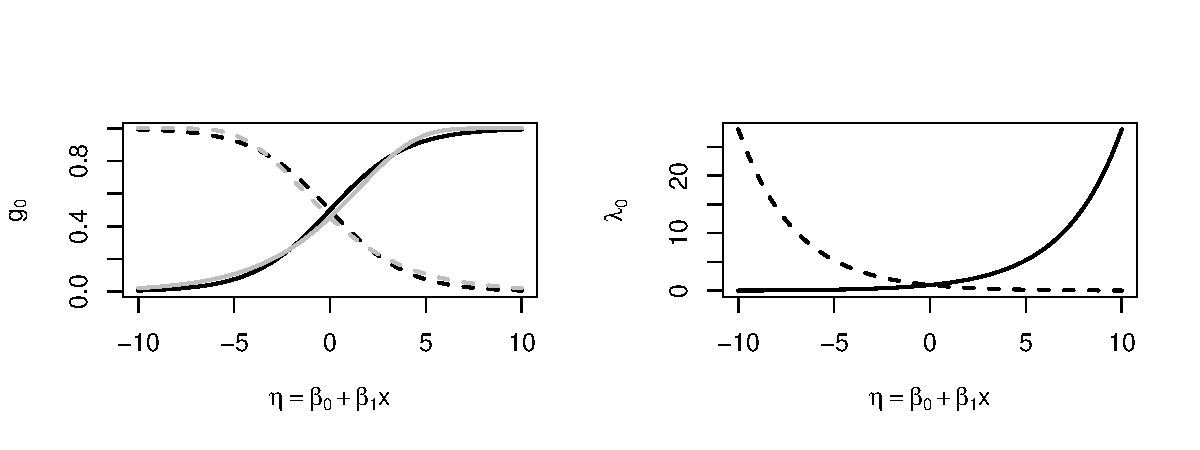
\includegraphics[width=12cm]{keepfigure/linkfuns.pdf}
\label{fig:ERdetfun.linkfuns}
\end{figure}

Dependence on more covariates is modelled by adding terms to the linear predictor: $\eta=\beta_0 + \beta_1 x_1 + \beta_2 x_2 + \cdots + \beta_m x_m$. 


\todo[inline]{Should we mention regression splines here, and add a plot explaining?}


The \texttt{secr} syntax for this follows the syntax for GLMs in \texttt{R}:
\noindent
{\small
\begin{svgraybox}
\texttt{
g0 \url{~} x1 + x2 + $\cdots$ + xm \\
lambda0 \url{~} x1 + x2 + $\cdots$ + xm \\
sigma \url{~} x1 + x2 + $\cdots$ + xm 
}
\end{svgraybox}
}
\noindent
The \texttt{secr} package automatically selects the log link for $\sigma$ and $\lambda_0$, and the logit link for $g_0$. Interaction terms and main effects with interactions can be added using ``\texttt{:}'' and ``\texttt{*}'', respectively, as with GLMs in \texttt{R}.



\section{Detector, occasion and stratum effects}

It is useful to separate variables that affect encounter rate and detection probability into two classes: those that need to be known throughout the survey region, and those that need to be known only at the detectors. In this section we deal with those that need to be known only at the detectors. This includes variables associated with occasions or strata, except in the case in which 


The effects on encounter rate and detection probability of variables associated with detectors are spatial only to the extent that detectors are located at specific points (or subregions - see Chapter~\ref{ch:arealine}) of space. Unlike variables affecting the distibution of activity centres, they are not inherently spatial. To use variables associated with detectors, we need only know the values of the variables at the detectors, not throughout the study region. 

Similarly, to use variables associated with occasions we need not know anything about what part of space was covered 

When there are differences between detectors that may make some more efficient than others ... (Hmmm, it is the data structure that is different between detector effects, occasion effects and stratum effects, not the model specification. Maybe these three sections need to be a running example, with code since there is not really anything methodological to say?)



\section{Effort effects}

The encounter rate function is the key to adjusting for changes in effort between traps, occasions or sessions. With it we already have a link function between the expected encounter rate $\lambda(d)$ or detection probability $p(d)$ on the one hand, and the time a detector operated ($T_{jkl}$ for detector $j$ on occasion $j$ in stratum $l$) on the other:

\section{Individual effects (behaviour and heterogeneity)}


\section{Habitat effects} %DLB
% knit_child('chapters/spatial-distribution.Rnw') %DLB
% knit_child('chapters/detprob-and-spatial.Rnw')  %DLB
% knit_child('chapters/explaining-diff-detection.Rnw') %DLB & EH
% knit_child('chapters/detector-types.Rnw')  %Ben
% knit_child('chapters/area-transect-detectors.Rnw')  %Ben
% knit_child('chapters/non-euclidian.Rnw')  %DLB
% knit_child('chapters/trend-models.Rnw')  %EH
% knit_child('chapters/survey-design.Rnw')  %EH
% knit_child('chapters/acoustics.Rnw')  %Ben
% knit_child('chapters/continuous-time.Rnw')  %Greg
% knit_child('chapters/open-popns.Rnw')  %DLB
% knit_child('chapters/unmarked-telemetry.Rnw')  %Ben
% knit_child('chapters/synthesis.Rnw')  %DLB

%%knit_child('chapters/chapter.Rnw')
%%knit_child('chapters/appendix.Rnw')


% Bibliography %
\bibliography{dlb}{}
\bibliographystyle{er-chicago}

\backmatter%%%%%%%%%%%%%%%%%%%%%%%%%%%%%%%%%%%%%%%%%%%%%%%%%%%%%%%
%%knit_child('chapters/glossary.Rnw')
%%knit_child('chapters/solutions.Rnw')

\index{Expected encounter rate|see{encounter rate}}
\index{Hazard rate|see{{\it also} encounter rate}}
\index{Capture function|see{Detection function}}
\index{Capture probability|see{Detection probability}}
\index{Detection probability|see{{\it also} Detection function}}
\index{Animal-level variables|see{{\it also} Heterogeneity}}
\index{Survey-level variables|see{{\it also} Heterogeneity}}

\printindex

%%%%%%%%%%%%%%%%%%%%%%%%%%%%%%%%%%%%%%%%%%%%%%%%%%%%%%%%%%%%%%%%%%%%%%

\end{document}





